\section{Minimização de $||\VECTOR{f}(\VECTOR{x})-\VECTOR{b}||_{\MATRIX{C}}^2+\alpha||\VECTOR{x}-\VECTOR{x}_{last}||_{\MATRIX{D}}^2$}


%\index{Minimização, métodos!Regularização de}
%\index{Problema inverso!Não linear}
\index{Minimização do erro quadrático!Não linear}%!Função $||\VECTOR{f}(\VECTOR{x})-\VECTOR{b}||_{\MATRIX{C}}^2+\alpha||\VECTOR{x}-\VECTOR{x}_{last}||_{\MATRIX{D}}^2$}

\begin{theorem}[Solução iterativa]\label{theo:minfxbCfxbaxoaxo}
Dados,
os vetores coluna $\VECTOR{x}\in \mathbb{R}^N$, $\VECTOR{b}\in \mathbb{R}^M$ e $\VECTOR{x}_{last}\in \mathbb{R}^N$,  
uma função $\VECTOR{f}:\mathbb{R}^{N} \rightarrow \mathbb{R}^{M}$, 
as matrizes diagonais $\MATRIX{C} \in \mathbb{R}^{M\times M}$ e $\MATRIX{D} \in \mathbb{R}^{N\times N}$, e 
definida a Eq. (\ref{eq:minfxbCfxbaxoaxo1}),
\begin{equation}\label{eq:minfxbCfxbaxoaxo1}
e(\VECTOR{x})=||\VECTOR{f}(\VECTOR{x})-\VECTOR{b}||_{\MATRIX{C}}^2+\alpha||\VECTOR{x}-\VECTOR{x}_{last}||_{\MATRIX{D}}^2,
\end{equation}
tendo em consideração que $\VECTOR{x}_{last}$ é uma constante equivalente a $\VECTOR{x}_{k-1}$
numa busca iterativa ou equivalente a $\VECTOR{p}$, 
se decidimos usar uma aproximação linear ao redor de $\VECTOR{p}$ em $\VECTOR{f}(\VECTOR{x})$; 
é dizer, o segundo somando na Eq. (\ref{eq:minfxbCfxbaxoaxo1}) 
procura minimizar $||\VECTOR{x}_{k}-\VECTOR{x}_{k-1}||_{\MATRIX{D}}^2$.


Se desejamos ter o ponto $\VECTOR{\hat{x}}$ que minimiza o escalar $e(\VECTOR{\hat{x}})$,
podemos achar este ponto usando iterativamente a Eq. (\ref{eq:minfxbCfxbaxoaxo2}),
onde  $\MATRIX{J}(\VECTOR{x})$ é a \hyperref[def:jacobian]{\textbf{matriz Jacobiana}}  de $\VECTOR{f}(\VECTOR{x})$.
\begin{equation}\label{eq:minfxbCfxbaxoaxo2}
\VECTOR{x}_{k}\leftarrow \VECTOR{x}_{k-1}-
\left[ \MATRIX{J}(\VECTOR{x}_{k-1})^{\transpose}\MATRIX{C} \MATRIX{J}(\VECTOR{x}_{k-1}) +\alpha\MATRIX{D} \right]^{-1}
 \left[\MATRIX{J}(\VECTOR{x}_{k-1})^{\transpose}\MATRIX{C}\left\{\VECTOR{f}(\VECTOR{x}_{k-1})-\VECTOR{b}\right\}\right],
\end{equation}
onde em cada iteração se tenta minimizar
\begin{equation}\label{eq:minfxbCfxbaxoaxo2:ex}
e_{k-1}(\VECTOR{x})  \equiv 
||\VECTOR{f}(\VECTOR{x})-\VECTOR{b}||_{\MATRIX{C}}^2+
\alpha||\VECTOR{x}-\VECTOR{x}_{k-1}||_{\MATRIX{D}}^2.
\end{equation}
Assim, $\VECTOR{\hat{x}}$ pode ser achado 
iniciando a Eq. (\ref{eq:minfxbCfxbaxoaxo2}) desde um $\VECTOR{x}_{0}$ qualquer, 
ate que $\VECTOR{x}_{k}$ seja muito próximo a $\VECTOR{x}_{k-1}$,
onde se declara que $\VECTOR{\hat{x}} \approx \VECTOR{x}_{k}$,
que corresponde a um mínimo\footnote{\label{ref:minfxxp}A
demostração pode ser vista na Prova \ref{proof:theo:minfxbCfxbaxod}.} de $e(\VECTOR{x})$,
sem aclarar se é local ou global.


\textbf{Considerções:}

\begin{itemize}
\item É interessante verificar sempre na Eq. (\ref{eq:minfxbCfxbaxoaxo2}) 
se  $\MATRIX{J}(\VECTOR{x}_{k-1}) = \MATRIX{0}$,
pois indica que existe\footref{ref:minfxxp} um ponto de inflexão 
(máximo, mínimo ou ponto de sela) em $e(\VECTOR{x}_{k-1})$;
consequentemente poderíamos ter achado um mínimo.
\item A busca iterativa da Eq. (\ref{eq:minfxbCfxbaxoaxo2}) é considerada falida quando 
$\MATRIX{J}(\VECTOR{x}_{k-1})^{\transpose}\MATRIX{C} \MATRIX{J}(\VECTOR{x}_{k-1}) +\alpha\MATRIX{D}$
não tem inversa.
\end{itemize}


\end{theorem} 


\begin{tcbattention}
\begin{itemize}
\item O Teorema \ref{theo:minfxbCfxbaxoaxo} pode ser usado para achar o vetor $\VECTOR{x}$
que minimize $||\VECTOR{f}(\VECTOR{x})-\VECTOR{b}||_{\MATRIX{C}}^2$, procurando 
em todo momento que na busca iterativa se minimize $||\VECTOR{x}_{k}-\VECTOR{x}_{k-1}||_{\MATRIX{D}}^2$,
\end{itemize}
\end{tcbattention}

%%%%%%%%%%%%%%%%%%%%%%%%%%%%%%%%%%%%%%%%%%%%%%%%%%%%%%%%%%%%%%%%%%%%%%%%%%%%%%%%
\subsection{Exemplos de minimização de 
$||\VECTOR{f}(\VECTOR{x})-\VECTOR{b}||_{\MATRIX{C}}^2+\alpha||\VECTOR{x}-\VECTOR{x}_{last}||_{\MATRIX{D}}^2$}


\begin{example}[Quando existem muitos mínimos locais e um
$\VECTOR{\hat{x}}$ que cumpre que $\VECTOR{f}(\VECTOR{\hat{x}}) \approx \VECTOR{b}$:]
\label{ex:minfxbCfxbaxqaxp1}
Conhecida um escalar $\alpha$, uma função $\VECTOR{f}(\VECTOR{x}) : \mathbb{R}^{2} \rightarrow \mathbb{R}^{3}$,
um ponto $\VECTOR{b}$ no contradomínio de $\VECTOR{f}(\VECTOR{x})$;
achar o valor $\VECTOR{\hat{x}}$ que minimize 
$||\VECTOR{f}(\VECTOR{x})-\VECTOR{b}||_{\MATRIX{C}}^2+\alpha||\VECTOR{x}-\VECTOR{x}_{last}||_{\MATRIX{D}}^2$;
sabendo que:
\begin{equation}
\VECTOR{b}=\begin{bmatrix}
1\\
1\\
2
\end{bmatrix},
\qquad 
\VECTOR{f}(\VECTOR{x})=\begin{bmatrix}
sin(\frac{x_1 5 \pi}{2})\\
sin(\frac{x_2 5 \pi}{2})\\
x_1+x_2
\end{bmatrix},
\qquad
\alpha=0.5.
\end{equation}
Com esta informação podemos calcular o jacobiano $\MATRIX{J}(\VECTOR{x})$ de $\VECTOR{f}(\VECTOR{x})$,
 e também escolher as matrizes $\MATRIX{C} \in \mathbb{R}^{3}$ e $\MATRIX{D} \in \mathbb{R}^{2}$, 
com elementos iguais à  matriz identidade. 
Assim, usando a Eq. (\ref{eq:minfxbCfxbaxoaxo2:ex}),
obtemos a superfície $e_{0}(\VECTOR{x})$ para um ponto inicial $\VECTOR{x}_0$ como mostra a Figura \ref{fig:ex:minfxbCfxbaxqaxp3:a}.
Podemos ver a resposta a este exemplo na Solução \ref{ex:minfxbCfxbaxqaxp3:sol1}.
\end{example}

\begin{SolutionT}[Relativa ao Exemplo \ref{ex:minfxbCfxbaxqaxp1}:]
\label{ex:minfxbCfxbaxqaxp3:sol1}
Se escolhemos o ponto inicial $\VECTOR{x}_0=[2.2183$ $2.2183]^{\transpose}$ e 
usamos iterativamente a Eq. (\ref{eq:minfxbCfxbaxoaxo2}), obtemos os valores 
de $\VECTOR{x}_k$ e $e_{k}(\VECTOR{x}_k)$, como mostra a Tabela \ref{table:ex:minfxbCfxbaxqaxp3},
onde se assume o final do processo iterativo quando $\VECTOR{x}_k \approx \VECTOR{x}_{k-1}$.
Assim, a aproximação iterativa conclui na resposta 
$\VECTOR{\hat{x}}\approx \VECTOR{x}_{4} =[1.0304\quad 1.0304]^{\transpose}$
com um erro $e_{4}(\VECTOR{\hat{x}})=6.6750~10^{-3}$;
este processo pode ser visto de forma gráfica na Figura \ref{fig:ex:minfxbCfxbaxqaxp3:b}.
\end{SolutionT}

\begin{table}[h!]
\centering
\begin{tabular}{|l|l|l|l|l|l|}
\hline
$k$ & 0 & 1 & 2 & 3 & 4 \\ \hline
$\VECTOR{x}_k$ & 2.2183 & 2.1656 & 1.2297 & 1.0676 & 1.0304 \\ 
~              & 2.2183 & 2.1656 & 1.2297 & 1.0676 & 1.0304 \\ \hline
$||\VECTOR{x}_k||$ & 3.1371 & 3.0627 & 1.7391 & 1.5099 & 1.4571 \\ \hline
$e_{k}(\VECTOR{x}_k)$ & 1.3855e+01 & 1.3151e+01 & 4.1187e+00 & 8.2579e-02 & 6.6750e-03 \\ \hline
\end{tabular}
\caption{Resposta iterativa do Exemplo \ref{ex:minfxbCfxbaxqaxp1}.}
\label{table:ex:minfxbCfxbaxqaxp3}
\end{table}
\begin{figure}[h!]
     \centering
     \begin{subfigure}[b]{0.49\textwidth}
         \centering
         \includegraphics[width=0.98\textwidth]{chapters/minimization-fx/mfiles/fxxx3/surfcfx3-0.eps}
         \caption{Superfície $e_0(\VECTOR{x})$.}
         \label{fig:ex:minfxbCfxbaxqaxp3:a}
     \end{subfigure}
     \hfill
     \begin{subfigure}[b]{0.49\textwidth}
         \centering
         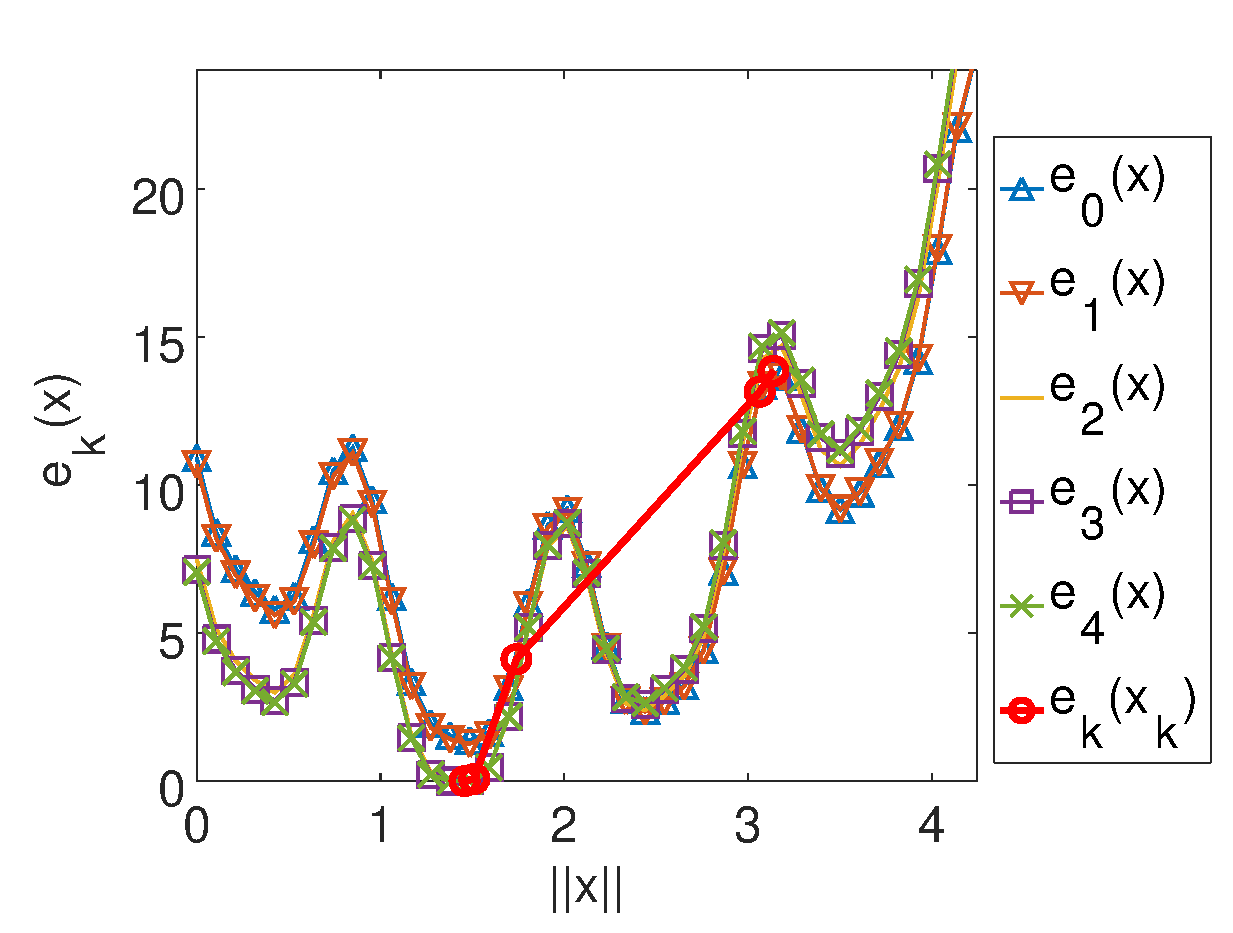
\includegraphics[width=0.98\textwidth]{chapters/minimization-fx/mfiles/fxxx3/plotfx3all.eps}
         \caption{Curva $e(\VECTOR{x})$ na direção $(1,1)$.}
         \label{fig:ex:minfxbCfxbaxqaxp3:b}
     \end{subfigure}
        \caption{Resposta gráfica do Exemplo \ref{ex:minfxbCfxbaxqaxp1}. }
        \label{fig:ex:minfxbCfxbaxqaxp3}
\end{figure}


